{\em Kuromasu} oder {\em Kurodoko} ist ein Rätsel, welches
von dem japanischen Rätselverlag Nikoli veröffentlicht wird.
In einem $n\times n$ Spielfeld sind in einzelnen Feldern Zahlen
vorgegeben.
Der Spieler muss nun Felder schwarz färben, er darf aber keine
Zahlfelder färben und schwarze Felder dürfen nicht benachbart sein.
Er muss dabei so vorgehen, dass
die Zahlfelder die Anzahl der weissen Felder in der gleichen Zeile
und Spalte bis zu einem schwarzen Feld oder dem Spielfeldrand angeben.
Hier ein Beispiel eines {\em Kuromasu}-Rätsels mit Lösung:
\begin{center}
\newboolean{blackfields}
\def\showfield{
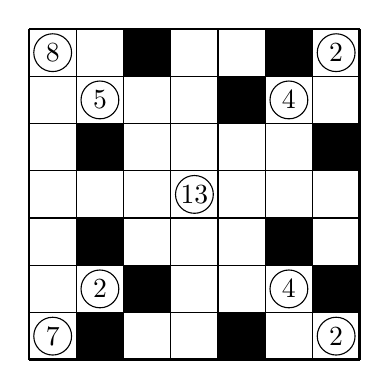
\begin{tikzpicture}[scale=0.6]
\foreach \x in {-0.5,0.5,...,6.5}{
	\draw ({\x},-0.5)--({\x},6.5);
}
\foreach \y in {-0.5,0.5,...,6.5}{
	\draw (-0.5,{\y})--(6.5,{\y});
}
\draw[line width=1pt] (-0.5,-0.5)--( 6.5,-0.5);
\draw[line width=1pt] (-0.5, 6.5)--( 6.5, 6.5);
\draw[line width=1pt] (-0.5,-0.5)--(-0.5, 6.5);
\draw[line width=1pt] ( 6.5,-0.5)--( 6.5, 6.5);

\node at (0,0) {$7$}; \draw (0,0) circle[radius=0.4];
\node at (1,1) {$2$}; \draw (1,1) circle[radius=0.4];
\node at (3,3) {$13$}; \draw (3,3) circle[radius=0.4];
\node at (5,5) {$4$}; \draw (5,5) circle[radius=0.4];
\node at (6,6) {$2$}; \draw (6,6) circle[radius=0.4];
\node at (0,6) {$8$}; \draw (0,6) circle[radius=0.4];
\node at (1,5) {$5$}; \draw (1,5) circle[radius=0.4];
\node at (5,1) {$4$}; \draw (5,1) circle[radius=0.4];
\node at (6,0) {$2$}; \draw (6,0) circle[radius=0.4];

\ifthenelse{\boolean{blackfields}}{
\fill (0.5,-0.5)--(1.5,-0.5)--(1.5,0.5)--(0.5,0.5)--cycle;
\fill (0.5, 1.5)--(1.5, 1.5)--(1.5,2.5)--(0.5,2.5)--cycle;
\fill (0.5, 3.5)--(1.5, 3.5)--(1.5,4.5)--(0.5,4.5)--cycle;
\fill (1.5, 0.5)--(2.5, 0.5)--(2.5,1.5)--(1.5,1.5)--cycle;
\fill (1.5, 5.5)--(2.5, 5.5)--(2.5,6.5)--(1.5,6.5)--cycle;
\fill (3.5,-0.5)--(4.5,-0.5)--(4.5,0.5)--(3.5,0.5)--cycle;
\fill (3.5, 4.5)--(4.5, 4.5)--(4.5,5.5)--(3.5,5.5)--cycle;
\fill (4.5, 1.5)--(5.5, 1.5)--(5.5,2.5)--(4.5,2.5)--cycle;
\fill (4.5, 5.5)--(5.5, 5.5)--(5.5,6.5)--(4.5,6.5)--cycle;
\fill (5.5, 0.5)--(6.5, 0.5)--(6.5,1.5)--(5.5,1.5)--cycle;
\fill (5.5, 3.5)--(6.5, 3.5)--(6.5,4.5)--(5.5,4.5)--cycle;
}{}
\end{tikzpicture}
}
\setboolean{blackfields}{false}
\showfield
\qquad
\setboolean{blackfields}{true}
\showfield
\end{center}
Kann eine nichtdeterministische Turing-Maschine in polynomieller Zeit
entscheiden, ob ein {\em Kuromasu}-Rätsel eine Lösung hat?

\thema{NP}
\thema{polynomieller Verifizierer}

\begin{loesung}
Das Problem ist sicher entscheidbar: es gibt nicht mehr als $2^{n\times n}$
mögliche Platzierungen von schwarzen Feldern, die man alle durchprobieren
kann um zu entscheiden, ob das Rätsel eine Lösung hat. 
Natürlich braucht man dazu exponentielle Zeit, mindestens auf einer 
deterministischen Turing-Maschine.

Eine nichtdeterministische Turing-Maschine kann die Lösbarkeit
genau dann in polynomieller Zeit entscheiden,
wenn es einen polynomiellen Verifizierer gibt.
Als Lösungszertifikat $c$ für den Verifizierer verlangen wir die schwarz
ausgefüllten Felder.
Der Verifikationsalgorithmus muss dann die folgenden Eigenschaften überprüfen:
\begin{center}
\begin{tabular}{r|p{10cm}|c}
&was&Komplexität\\
\hline
1&Für jedes schwarze Feld (maximal $O(n^2)$) verifiziere, dass keines der Nachbarfelder
schwarz ist&$O(n^2)$\\
2&Für jedes Zahlfeld (maximal $O(n^2)$)
zähle die Anzahl Felder in der gleichen Zeile
und Spalte bis zum Rand oder zum nächsten schwarzen Feld (je
maximal $O(n)$) und
verifiziere, dass sie mit der gegebenen Zahl übereinstimmt&$O(n^3)$\\
\hline
&Total&$O(n^3)$
\end{tabular}
\end{center}
Der Verifikationsalgorithmus kann als mit Hilfe des Lösungszertifikates in
maximal $O(n^3)$ Schritten, also in polynomieller Zeit, entscheiden,
ob $c$ eine Lösung ist.
Damit ist gezeigt, dass ein polynomieller Verifizierer existiert.
\end{loesung}

\begin{diskussion}
Jonas Kölker hat 2012 bewiesen, dass Kurodoko NP-vollständig ist:
{\em Kurodoko is NP-Complete}, Journal of Information Processing,
vol.~20 (2012), no.~3, pp.~694-706,
\url{https://doi.org/10.2197/ipsjjip.20.694}.
\end{diskussion}

\begin{bewertung}
Entscheidbarkeit ({\bf E}) 1 Punkt,
Verifizierer ({\bf V}) 1 Punkt,
Zertifikat ({\bf Z}) 1 Punkt,
Algorithmus ({\bf A}) 1 Punkt,
Laufzeitschätzung ({\bf L}) 1 Punkt,
Schlussfolgerung ({\bf S}) 1 Punkt.
\end{bewertung}

